\documentclass[11pt]{article}
\usepackage[utf8]{inputenc}
\usepackage[T1]{fontenc}
\usepackage{amsmath}
\usepackage{amsfonts}
\usepackage{amssymb}
\usepackage[version=4]{mhchem}
\usepackage{stmaryrd}
\usepackage{graphicx}
\usepackage[export]{adjustbox}
\graphicspath{ {./images/} }

\begin{document}
Volatility Arbitrage

Trading on the basis of prices is as old as money itself. The concept of explicitly trading on the basis of asset price volatility is relatively new. Volatility arbitrage is any strategy that attempts to earn a superior and riskless profit based on prices that explicitly depend on volatility.

\section*{Volatility and Vega Overview}
Any security that contains a nontrivial option feature may be viewed as having a direct relationship between its price and the volatility of the underlying asset, holding all other values constant. Often multiple security prices depend on the same underlying asset volatility (or related asset volatilities). Examples include options on the same asset that differ with regard to strike price, expiration date, type of option (e.g., European, American, Bermuda, range, and knockout), and being calls or puts. This permits traders to speculate on the relative performance of the multiple securities with option characteristics and with the same underlying asset.

A key concept in volatility arbitrage and options in general is vega. Vega is a measure of the risk of a position or an asset due to changes in the volatility of a price or rate that helps determine the value of that position or asset. For example, in the case of an option, vega is the first derivative of the option price with respect to the implied volatility of the returns of the asset underlying the option. Vega risk is the economic dispersion caused by changes in the volatility of a price, return, or rate.

A key distinction in volatility involves differences between implied volatility, anticipated volatility, and realized volatility. In all three cases, volatility is defined as the standard deviation of returns. Implied volatility, as discussed earlier, is the level of volatility in an option's underlying asset inferred by the current price of the option based on a particular option pricing model. Implied volatility is a mathematical computation performed by searching for the level of asset volatility that, when inserted into a specified option pricing model, generates a model price that equals the current market price of the option. Anticipated volatility is the future level of volatility expected by a market participant. Realized volatility, as discussed previously, is a statistically based estimate of the actual historical volatility experienced in the marketplace. Market participants often develop anticipations of volatility based on observations of realized volatility. They then compare the anticipated volatility with the implied volatility of options, taking long option positions when their anticipations of volatility exceed the implied volatility and short option positions when their anticipations of volatility are lower than the implied volatility.

It is especially important in discussing volatility arbitrage funds to be careful regarding the use and meaning of the term volatility. Outside investments, volatility is interpreted as simply indicating dispersion. Within investments, volatility is typically used specifically as and synonymously with standard deviation. However, in the area of volatility derivatives and variance derivatives, the terminology is evolving, and it is not always clear that volatility refers solely to standard deviation or that variance derivatives reference only variance.

Sinclair presents some stylized observations regarding volatility, many of which are key assumptions behind some volatility arbitrage portfolio strategies and risk management techniques:

\begin{enumerate}
  \item Volatility is not constant, but it mean-reverts, clusters, and has long memory. As such, many traders will model volatility using a regime-switching model.

  \item Volatility tends to stay low for some extended period of time until a market shock occurs and volatility transitions to a higher level for some period of time.

  \item The volatility of volatility can be high, but in the long run, volatility tends to revert toward some long-term average level.

  \item In equity markets, volatility tends to increase as price levels decline.

  \item Volatility tends to rise more quickly in response to stock prices falling than it falls in response to stock prices rising. ${ }^{1}$ Euan Sinclair (2013), Volatility Trading (Hoboken, NJ: John Wiley \& Sons).

\end{enumerate}

The final two observations may partially explain volatility skew levels, in which equity put option prices often trade at higher implied volatility levels than equity call option prices of similar deltas.

\section*{Instruments Used by Volatility Arbitrage Funds}
Managers of volatility arbitrage funds have substantial latitude in the choice of assets to trade in their funds. Broadly speaking, these funds may have positions in any instrument with volatility exposure. These assets include exchange-traded options, warrants, convertible bonds, other bonds with embedded options, over-thecounter (OTC) options, and OTC variance swaps. In recent years, a robust exchange-traded market has arisen in volatility futures and options, trading specifically on the Chicago Board Options Exchange (Cboe) Volatility Index (VIX), which measures the implied volatility of options on the S\&P 500 Index. A given volatility arbitrage fund may focus on these assets within one market, such as equities, while others may mix instruments across currency, debt, equity, credit, and commodity markets. In addition to holding assets with option characteristics, volatility arbitrage funds also hold assets without option characteristics in order to hedge or reduce their net exposure to moves in the underlying markets. The simplest examples of positions taken by volatility arbitrage funds involve exchange-traded options and warrants, whose performance is tied to price moves in single-equity securities or futures contracts in the equity, commodity, currency, or debt markets. In order to focus trading on volatility, traders follow a strict delta-hedging process to hedge away moves in the underlying market.

Bonds with embedded options can also be attractive to managers of volatility arbitrage funds. Convertible bonds have an embedded long call option on the issuer's stock, whereas mortgage-backed securities (MBS) are short a put option on interest rates (which is a short call option on bond prices), meaning borrowers are allowed to prepay their mortgages without penalty. Complex or illiquid securities may offer higher expected returns and more frequent opportunities from mispricing. For example, valuation of MBS requires assumptions regarding future interest rate paths and volatility, as well as the potential prepayment rates of the borrowers under various interest rate scenarios.

Variance swaps are forward contracts in which one party agrees to make a cash payment to the other party based on the realized variance of a price or rate in exchange for receiving a predetermined cash flow. Variance swaps are OTC products and are commonly traded by volatility arbitrage funds. These contracts offer cash flows based on the annualized variance in the returns on a referenced asset. In a variance swap, one party (the variance buyer) pays a predetermined variance (referred to as a swap strike price or strike variance) and receives realized variance. The counterparty (the variance seller) has the opposite cash flow exposure, receiving a fixed variance and paying realized variance. The amount of the net cash flow is the difference between the realized variance and the strike variance multiplied by the variance notional value of the contract. The variance notional value of the contract simply scales the size of the cash flows in a variance swap. The annualized variance is simply the squared value of the annualized standard deviation. At maturity, a variance swap pays off according to the following formula:

Variance Swap Payoff $=$ Variance Notional Value

$\times($ Realized Variance - Strike Variance)

For example, consider a 30-day variance swap on the returns of the S\&P 500 Index with a variance notional value of $\$ 100,000$. The strike variance of the swap is 4.00 (corresponding to a $4 \%$ annualized variance). After the 30 -day reference period is observed, the realized annualized variance in the index is, for example, 4.50 . The payoff of the variance swap would be as follows:

$$
\text { Variance Swap Payoff }=\$ 100,000 \times(4.50-4.00)=\$ 50,000
$$

A volatility swap mirrors a variance swap except that the payoff of the contract is linearly based on the standard deviation of a return series rather than the variance. In a volatility swap, the payoff is determined by multiplying the spread between the realized volatility and the strike volatility by the vega notional value. Similar to the variance notional value, the vega notional value of a contract serves to scale the contract and determine the size of the payoff in a volatility swap. The vega notional value provides a simple payoff formula for volatility swaps:

Volatility Swap Payoff $=$ Vega Notional Value


\begin{equation*}
\times(\text { Realized Volatility }- \text { Strike Volatility }) \tag{1b}
\end{equation*}


For example, a volatility swap with a vega notional value of $\$ 50,000$ would pay off $\$ 100,000$ if the realized volatility was 22.00 when the strike volatility was 20.00 .

The payoff to a variance swap in Equation 1a is often expressed using an expression that includes the vega notional value in place of the variance notional value. The variance notional value is equal to the vega notional value divided by 2 times the square root of the strike variance. In other words, the vega notional value is equal to the variance notional value multiplied by 2 times the square root of the strike variance. Inserting the formula for variance notional based on vega notional value into Equation 1a offers the following more common but less simple and less intuitive payoff formula:

EQUATION EXCEPTION LIST:

$$
\text { Variance Swap Payoff }=\frac{\text { Vega Notional Value } \times(\text { Realized Variance }- \text { Strike Variance })}{2 \times \sqrt{\text { Strike Variance }}}
$$

It should be noted that the exact computation methods are specified in the documentation but are not perfectly standardized.

The attraction to variance swaps is that they offer a pure play on asset return variance without exposure to the direction of moves in the underlying instrument. To speculate on the spread between implied and realized volatility in the exchange-traded options market without variance swaps, traders need to buy one set of options, sell another set of options, and frequently rebalance the hedges to keep exposures to the underlying markets close to delta-neutral. Options can be complex, exposing traders not only to volatility exposure (vega risk) but also to moves in the underlying assets (delta and gamma risk). Variance swaps give pure volatility exposure without the directional risk of moves in the underlying assets, which eliminates the obligation to continually rehedge the delta risk of the portfolio. As OTC products, variance swaps create counterparty risk, which must be monitored at all times.

\section*{Risks of Exchange-Traded versus OTC Derivatives}
Standardized, exchange-traded derivatives and other instruments can be less risky than some OTC instruments. Exchange trading is physically or electronically centrally located. Each instrument traded on the exchange is listed by the exchange, a process that specifies and unifies the characteristics of each instrument. OTC instruments are typically traded by investment banks and fixed-income brokerage houses and vary from being uniform (e.g., shares of common stock) to being unique (e.g., currency swaps with specific delivery dates). Generally, there are three major risks that positions in OTC-traded instruments have relative to positions in exchange-traded instruments:

\begin{enumerate}
  \item Exchange-traded instruments tend to offer less counterparty risk. Options involve an ongoing obligation by the party with the short position (the option writer) to pay cash or deliver assets to the other party (the option owner). Swaps offer an ongoing obligation by each party to pay cash to the other party. Counterparty risk is the potential dispersion in economic outcomes caused by the potential or actual failure of the other side of a contract to fulfill its obligations. In this case, the investor and the swap dealer have counterparty risk that the other might fail to fulfill the contract. By contrast, exchange-traded derivatives have clearinghouses that back the obligations of the members associated with each listed security.
\end{enumerate}

Clearinghouses have capital and the incentives and powers to demand collateral and creditworthiness of market participants, greatly mitigating the concerns with regard to the integrity of each contract. Moreover, clearinghouses diversify risk away from a single dealer and spread the risk across multiple members (or broker-dealers), making it less exposed to a single counterparty.

\begin{enumerate}
  \setcounter{enumi}{1}
  \item Exchange-traded instruments tend to offer higher price transparency and less pricing risk. Price transparency is information on the prices and quantities at which participants are offering to buy (bid) and sell (offer) an instrument. Pricing risk is the economic uncertainty caused by actual or potential mispricing of positions. For example, complex and unique derivative OTC instruments might have no information on prices other than estimations derived through complex models or price indications offered by dealers. Conversely, exchange-traded instruments have easily observable prices at which trades have taken place, and bids and offers of prices at which participants are currently willing to transact.

  \item Exchange-traded instruments tend to offer higher liquidity. Owing to price transparency, standardization of the terms of a security, reduced counterparty risk, and centralized trading, exchange-traded instruments tend to offer substantially higher liquidity than do OTC instruments. Liquidity provides market participants with the ability to manage their risks more effectively by being able to transact without substantially affecting market prices.

\end{enumerate}

These three major risks were vividly illustrated during the global financial crisis of 2007 to 2009 . For example, counterparty risk was experienced in 2008 . Traders with counterparty risk exposure to particular subsidiaries of Lehman Brothers were not paid the gains on their derivative positions when Lehman Brothers defaulted. Further losses to counterparties were avoided when the U.S. government was called on to guarantee the payment of OTC derivative contracts that had been sold by American International Group, Inc.

The price transparency of exchange-traded products facilitates the use of mark-to-market pricing. Marking-to-market refers to the use of current market prices to value instruments, positions, portfolios, and even the balance sheets of firms. The use of OTC derivatives often partially or fully relies on pricing based on a mark-tomodel methodology. Marking-to-model refers to valuation based on prices generated by pricing models. The pricing models generally involve two components. An instrument that is not frequently traded, and therefore does not offer price transparency, is modeled as being related to one or more market prices, rates, or factors. The current values of the determinants of the model price are then input into the model to approximate the value of the instrument. Thus, marking-to-model requires the specification of a model and its inputs. A problem with marking-to-model is that different investors holding similar securities may report widely different valuations to their investors based on the assumptions underlying their proprietary pricing model or the inputs used. In comparison, exchange-traded products are marked-to-market, wherein all investors value their holdings at a single, exchange-disseminated price.

\section*{Volatility Arbitrage Strategies}
An essential concept to understanding volatility arbitrage strategies is vega. As previously defined, vega is the sensitivity of an option or a security with an embedded option to changes in the volatility of the price or the returns of the asset underlying the option. A long position in an option has a positive vega, a short position in an option has a negative vega, and a position without option characteristics has a vega of zero. Note that vega indicates the sensitivity of an asset to changes in volatility assuming all other values are held constant. In practice, when volatility changes, there are usually changes in price levels.

Volatility arbitrage funds trade a variety of assets, typically taking long positions in instruments in which volatility is underpriced (or underestimated), and short positions in instruments in which volatility is overpriced (or overestimated). Other market risks are often hedged out, leaving the fund with less directional risk to the underlying markets. Instead, the positions are exposed to volatility risk and correlation risk. Volatility risk is dispersion in economic outcomes attributable to changes in realized or anticipated levels of volatility in a market price or rate. Correlation risk is dispersion in economic outcomes attributable to changes in realized or anticipated levels of correlation between market prices or rates.

As markets move, the fund manager needs to continue to implement rebalancing trades to remain delta-neutral. These rebalancing trades are profitable for long volatility positions that have positive gamma and unprofitable for short volatility positions that have negative gamma. However, positions long in vega are usually exposed to theta risk (negative theta), such that as time passes in a period with low asset volatility, the positions decline in value.

There are two main types of volatility arbitrage funds: those that are market (volatility) neutral and those that are intentionally exposed-typically long-to volatility. An example of a long volatility strategy is a variance buyer in a variance swap. The position either generates a payoff or requires a payoff based entirely on realized volatility. Long volatility funds can provide valuable tail risk protection during times of rising volatility, when markets are likely to decline. Market-neutral volatility funds seek to earn a profit without exposure to changes in volatility levels. An example of a market-neutral volatility strategy would be offsetting positions in two options with different implied volatilities in the same or similar underlying assets. The profit or loss is primarily driven by changes in the relationship between the two implied volatilities rather than the level of volatilities.

\section*{Market-Neutral Volatility Funds}
The most common strategy pursued by market-neutral volatility funds has been to make the assumption that there is an arbitrage opportunity between the higher implied volatility and the lower realized volatility for some options. In other words, the assumption is that some options are overpriced, and the trading strategy involves writing those options. The fund hedges the overall exposure of short positions in the options perceived as being overpriced by taking one or more offsetting positions in securities deemed to be more appropriately priced. As an example, a fund may sell equity index options and hedge the risk with a dynamically adjusted replicating portfolio of equity index futures that approximates the returns of the realized variance of the underlying equity market.

One example of why implied volatility of some options might consistently overestimate realized volatilities involves out-of-the-money index puts. Due to the demand for index put options to serve as protection from downside risk, implied volatility of out-of-the-money index put options is frequently believed to trade higher relative to realized volatility. The spread between implied and realized volatility compensates volatility sellers for providing insurance against rising volatility and falling markets. This spread is likely to continue as long as sellers of index volatility continue to demand a risk premium for providing insurance coverage to other market participants and as long as insurance buyers continue to be willing to pay for the protection.

\section*{Challenges of Estimating Dispersion}
Care is necessary in interpreting measures of dispersion in the context of volatility derivatives. First, there are numerous conventions for calculating dispersion, so implied versus realized computations should be compared only when both series are calculated with consistent methodologies. Second, the payoff of variance swaps is linearly related to the square of volatility (i.e., variance is the square of standard deviation) and is therefore highly nonlinear relative to volatility, or standard deviation. Estimates of implied standard deviation based on observation of derivative prices with payouts linearly related to variance, such as those shown in Equation 2, are biased as predictors of volatility.

Suppose that the realized volatility of an asset has exactly six equally likely outcomes: $1 \%, 2 \%, 3 \%, 4 \%, 5 \%$, or $6 \%$. The expected value of the volatility is $3.5 \%$. Now consider the same dispersion expressed in term of variance: $0.0001,0.0004,0.0009,0.0016,0.0025$, and 0.0036 . The expected value of the variance is approximately 0.00152. The volatility corresponding to this variance is approximately $3.9 \%$. The square root of the expected variance differs substantially from the expected volatility (standard deviation). Special care should be taken in comparing volatility computations and variance computations.

\section*{Tail Risk Strategies}
Tail risk is the potential for very large loss exposures due to very unusual events, especially those associated with widespread market price declines. Entities with undesirably high exposures to tail risk may seek protection from tail risk that is often termed portfolio insurance. Portfolio insurance is any financial method, arrangement, or program for limiting losses from large adverse price movements. Portfolio insurance can be provided through dynamic trading strategies that hedge losses, such as taking short positions in corresponding futures contracts that are adjusted in size based on market levels. Portfolio insurance can also be provided by establishing positions in investments that thrive during periods associated with tail risk. A straightforward solution is to purchase long positions in put options that\\
are very far out-of-the-money. The problem with buying puts that are far out-of-the-money is that they are often viewed as being priced very high. In other words, market participants often view those options as having implied volatility that substantially exceeds expectations of realized volatility. Purchasing out-of-the-money put options at high implied volatilities can be a substantial drag on portfolio performance when, as usually happens, there are no crises and the options expire worthlessly. The explanation for the high implied volatilities is that there is tremendous demand from institutional investors to hold the options for protection against tail risk and a limited number of market participants with the financial resources and desire to provide such protection by writing the puts.

Tail risk strategies may be viewed as attempts to fill the market need for portfolio protection without the potentially large costs of purchasing put options that regularly expire worthlessly and that therefore generate losses during normal market conditions. Some volatility arbitrage funds attempt to design tail risk strategies that earn substantial profits during times of stress, panics, crises, and widespread losses, and generate only small losses or perhaps even small gains during most other market conditions.

For example, a fund may develop a strategy of taking long positions in options with implied volatilities that are deemed low and writing options with implied volatilities that are deemed high. The fund may believe that these particular option positions will permit large profits in the event of a major market decline while having very limited losses in normal markets. It should be noted that option-like payoffs can be attempted using non-option securities through dynamic rebalancing strategies. For example, a strategy that buys additional assets when asset prices rise and liquidates positions when asset prices decline exhibits high upside potential and low downside risk, similar to that of a long call option position. However, such strategies are likely to fail during periods of extreme market stress or over times when markets are closed, since prices and volatility can jump before the necessary dynamic adjustments can be implemented.

The payoff profile of tail risk funds is designed to be negatively correlated to price levels in major markets, especially equity and credit markets. As equity markets decline and credit spreads widen, volatility and correlation tend to increase. Tail risk funds that can profit during these times of crisis can serve as a hedge to the risk exposures of traditional equity and credit market investors. These tail risk funds are used by investors who mix the tail risk strategies into portfolios with substantial long exposure to equity and credit investments to provide a combined portfolio with the goal of profitability during normal market conditions and little or no downside risk during periods of market stress.

Funds that offer the attractive payoff profile of providing tail risk protection may be relatively delta-neutral for small changes in market conditions but lose their delta neutrality for large changes so that they can generate gains during large market drops. In other words, the strategies are long gamma. The strategies are also long vega, since they benefit from rising levels of volatility.

Correlation among assets is a crucial issue in tail risk strategies. During normal market conditions, it is observed that, for example, stocks have modest correlation with each other, simultaneously rising or falling by different amounts. However, during periods of market stress, it is often said that correlations go to one. The term correlations go to one means that during periods of enormous stress, stocks and bonds with credit risk decline simultaneously and with somewhat similar magnitudes. However, some analysts prefer to describe this phenomenon by breaking movements in risky assets into market risks and idiosyncratic risks. During normal market conditions, price changes due to idiosyncratic factors are not dominated by changes due to market factors, so correlations between risky assets are modest. The reason is that idiosyncratic movements are uncorrelated by definition. However, during periods of stress, the market factors dominate the idiosyncratic factors, causing risky assets to have highly correlated returns. The reason is that the market-related movements of the individual assets are perfectly correlated by definition. The point of this analysis is that the underlying correlations, parameters, and processes do not change during periods of market stress. Rather, during these periods of stress, market factors experience larger volatility and therefore exert larger effects than do idiosyncratic factors. However, not all assets have returns that increase in correlation with each other during a market crisis. There are defensive assets that have historically been able to maintain their value or even post profits in a market crisis, actually moving toward negative one in terms of correlation with risky assets. These defensive assets may include long put options, long call options on volatility, sovereign debt, and even some hedge fund strategies, such as global macro or managed futures.

Tail risk funds tend to be less focused on pure arbitrage and therefore take positions across markets, attempting to sell overpriced volatility and buy underpriced volatility in whatever markets can be found. If tail risk strategies are able to post large gains during times of market crisis, owners of these funds gain access to valuable cash when other investors may have constrained liquidity in their portfolios. This improved cash position can provide substantial benefits to investors. Investors may be able to avoid losses due to liquidity concerns, such as by being able to fund capital calls to real estate and private equity funds without selling equity and credit investments after sharp market declines. The cash generated from the tail risk portfolio can also be used to opportunistically purchase assets at fire-sale prices from distressed investors who need to raise cash. Although the benefits of a tail risk fund are clear, the challenge to the fund manager is to provide protection during crisis markets without paying too much in option premiums during normal market conditions, which can persist for a very long time. In essence, the strategy attempts to mimic the payouts to out-of-the-money put protection at a lower cost through the implementation of sophisticated trading strategies.

\section*{The Dispersion Trade}
The classic dispersion trade is a market-neutral short correlation trade, popular among volatility arbitrage practitioners, that typically takes long positions in options listed on the equities of single companies and short positions in a related index option. For example, a fund may buy options on 50 different large-capitalization, U.S.listed firms and take a short position in options listed on the S\&P 500 Index. Typically, the goal is to create a basket of options on individual assets that mimics the composition of the index closely, perhaps by matching the industry weights of the portfolio.

The key to the dispersion trade is the relationship between a portfolio of options and a single option on a portfolio. That relationship is driven by volatility, which in turn is driven by correlations across assets. Portfolio variance is lower when the constituent stocks have lower volatility and lower correlation with each other. Conversely, as the correlations between stocks rise, portfolio variance increases, as there are fewer stocks experiencing offsetting price moves. Thus, the relative returns of options on indices and options on individual assets are driven by changes in the anticipated correlation among the assets. In practice, individual assets are not highly correlated with each other, so the realized volatility of individual assets tends to be substantially higher than the realized volatility of a related index. Therefore, the implied volatilities of options on individual assets tend to be higher than the implied volatility of an option on a related index. Equation 3 expresses the variance of the return of a portfolio as depending on the variance of the constituent assets and their correlations:


\begin{equation*}
V\left(R_{p}\right)=\sum_{i=1}^{n} \sum_{j=1}^{n} w_{i} w_{j} \sigma_{i} \sigma_{j} \rho_{i j} \tag{3}
\end{equation*}


where $V\left(R_{p}\right)$ is the variance of the portfolio, $R_{p}$ is the return on the portfolio, $n$ is the number of assets in the portfolio, $w_{i}$ is the weight of asset $i$ in the portfolio, $\Sigma_{i}$ is the standard deviation of returns for asset $i$, and $\rho_{i j}$ is the correlation coefficient between returns on assets $i$ and $j$. When $i=j, \rho_{i j}=1$.

In summary, correlation drives the magnitude of the differences between the volatilities of individual assets and portfolios. Lower values of correlation generate lower portfolio risk through diversification, whereas higher correlation inhibits diversification. Dispersion trades are speculations on correlation. The classic dispersion trade is that realized correlations between assets will be lower than the correlation implied by the pricing of index options relative to options on individual assets. Therefore, the classic dispersion trade is referred to as a short correlation trade because the trade generates profits from low levels of realized correlation and losses from high levels of realized correlation.

\section*{Profit and Loss on Dispersion Trades}
Profits from the classic dispersion trade (long individual asset options and short index options) are the greatest during times of declining correlation, and losses occur when correlations rise significantly. The logic and terminology of dispersion trades parallel those of most option trading. Fund managers focus on the difference between implied correlations and realized correlations rather than implied volatility and realized volatility. The ideal condition for a classic dispersion trade is when implied correlation between stocks is high and the fund manager can consistently predict when realized correlation is going to be lower. Conversely, traders may implement a reverse dispersion trade-buying the index options and writing the single stock options-when implied correlation is lower than the trader's expectation for realized correlation.

As an example, consider a basket of four stocks (stocks A, B, C, and D), each of which is one-quarter of the weight of an index. Begin by assuming that the classic dispersion trade is implemented by purchasing equal quantities of four call options that are near-the-money on the four individual stocks and writing call options on the index. The short position in the index calls is assumed to have an aggregated magnitude in terms of underlying asset value equal to the sum of the underlying asset values of the four individual options. Assume that the options have three months to expiration, that the implied correlation among the four individual stocks in the index is equal to 0.30 , and that the implied annualized volatilities of the individual options are all 0.40 .

The profits from the classic dispersion trade are high when the realized correlation is lower than the implied correlation (i.e., when realized volatilities on individual stocks are relatively high, and realized volatilities on the index are relatively low). For example, if stocks A and B rise in value by $50 \%$ during the lifetime of the options, and stocks $C$ and $D$ fall by $50 \%$ over the same time period, the profitability of the single stock call options on $A$ and $B$ is extremely high due to the large upward movement in the underlying stocks. The call options on stocks $C$ and $D$ are worthless. The positive gamma ensures that the profits on the options on $A$ and $B$ will exceed the losses on C and D, so that the aggregated long positions in the individual options perform very well. Note that although the stocks experienced large moves, the stock market index was unchanged, as the positive returns on $A$ and $B$ were offset by the negative returns on $C$ and $D$. The correlations among the assets in the index were a mix of positive and negative values. Since the stock market index was unchanged, the index options that had been written expire worthless, making for an extremely profitable dispersion trade. In a nutshell, the realized correlation was lower than the implied correlation.

Note that the dispersion trade in this example would also be very profitable using put options instead of call options. In that case, the put options on C and D would pay off well, while the losses on the put options on A and B would be limited. Further, the short position in the index put would generate a profit by expiring worthlessly. The reason that either calls or puts would generate profits is that the market remained unchanged.

Having analyzed the profitability of the classic dispersion trade, it is easy to compute the profitability of the reverse trade (buying the index option and writing the individual options). The reverse trade would have lost money using calls or puts, since the classic trade and reverse trade are mirror images of each other. Delta neutrality can be pursued either by mixing calls and puts (i.e., using straddles and strangles) or by hedging with the underlying assets of the options.

Now consider what would happen in a classic dispersion trade using call options if all four stocks moved up 50\% together or down 50\% together. In other words, what would happen if the realized correlation was 1.00 ? If all four stocks rose $50 \%$, all four call options on the individual stocks, as well as the index option, would pay approximately $50 \%$ of the value of the underlying assets; and given the weighting assumptions, the aggregated payoff would be zero, due to the loss on the short position in the index option. If all four stocks fell by $50 \%$, all four call options as well as the index option would expire worthlessly, and the aggregated payoff would again be zero. However, the classic trade would generate losses in either scenario, since the positions required an initial outlay of capital. The reason that establishing the positions required an initial outlay was that the options on the individual stocks cost more than the income the writing of the index option generated; this is because the implied volatilities of the individual options exceeded the implied volatility of the index, which is always the case when the implied correlation is less than one.

\section*{Summary of Five Volatility Arbitrage Risks}
The Summary of Volatility Arbitrage Risks exhibit below summarizes the risks of various volatility arbitrage strategies. Note that five major determinants of performance are the returns in the underlying market, correlation, volatility, counterparty solvency, and market liquidity. Knowledge of the risks related to volatility arbitrage performance is essential.

Summary of Volatility Arbitrage Risks

\begin{center}
\begin{tabular}{|ll|}
\hline
Risk & Effect \\
\hline
Underlying markets: equity, credit, & Market-neutral volatility arbitrage funds seek to minimize risks to underlying markets through delta-hedging \\
commodity, currency, and interest rates & trades. Tail risk funds may retain substantial exposure to changes in underlying markets. \\
Correlation & Market-neutral and dispersion trades are short correlation trades that seek to benefit from market convergence. \\
 & Tail risk funds are long correlation trades, seeking to benefit during times of market crisis. \\
Volatility & Market-neutral funds try to minimize volatility exposure, seeking to take offsetting long and short volatility \\
 & positions. Tail risk funds typically benefit during times of rising volatility. \\
Counterparty & Exchange-traded positions have minimal counterparty risks, whereas OTC trades can incur substantial \\
 & counterparty risks, which need to be monitored and controlled. \\
Liquidity & Some positions, especially those in credit instruments and structured products, incur substantial liquidity risks. \\
 & Trades placed on exchange-traded markets have much lower liquidity risks. \\
\end{tabular}
\end{center}

\section*{Key Observations Regarding Historical Returns of Relative Value Volatility Funds}
Monthly returns to relative value volatility funds are observed from January of 2009 to December of 2021, for a total of 144 observations. Statistical Summary of Returns provides univariate return statistics and partial autocorrelations of returns in the top panel, and a histogram of returns in the bottom panel. Due to a shorter track record, the following statistics mix data from the HFRX and HFRI Relative Value: Volatility indices.

\begin{center}
\begin{tabular}{lcc}
\hline
\multicolumn{1}{c}{}\begin{tabular}{c}
Index (Jan. 2009- \\
Dec. 2021) \\
\end{tabular} & \begin{tabular}{c}
HFRX Relative Value: \\
Volatility Index \\
\end{tabular} & \begin{tabular}{c}
MSCI World \\
Equity \\
\end{tabular} \\
\hline
Annualized Arithmetic Mean & $3.0 \%$ & $12.8 \%$ \\
Annualized Standard Deviation & $4.8 \%$ & $15.1 \%$ \\
Annualized Semivolatility & $5.0 \%$ & $10.7 \%$ \\
Annualized Median & $1.8 \%$ & $5.8 \%$ \\
Skewness & -1.8 & -0.4 \\
Excess Kurtosis & 5.1 & 0.9 \\
Sharpe Ratio & 0.1 & 0.7 \\
Sortino Ratio & 0.1 & 1.0 \\
Annualized Geometric mean & $2.8 \%$ & $11.7 \%$ \\
First-Order Autocorrelation & 0.1 & 0.0 \\
Annualized Standard Deviation & $4.1 \%$ & $11.5 \%$ \\
(Adjusted for Autocorrelation) & $3.2 \%$ & $12.8 \%$ \\
Maximum & $-6.5 \%$ & $-13.2 \%$ \\
Minimum & $-8.2 \%$ & $-21.1 \%$ \\
Max Drawdown &  &  \\
\hline
\end{tabular}
\end{center}

\begin{center}
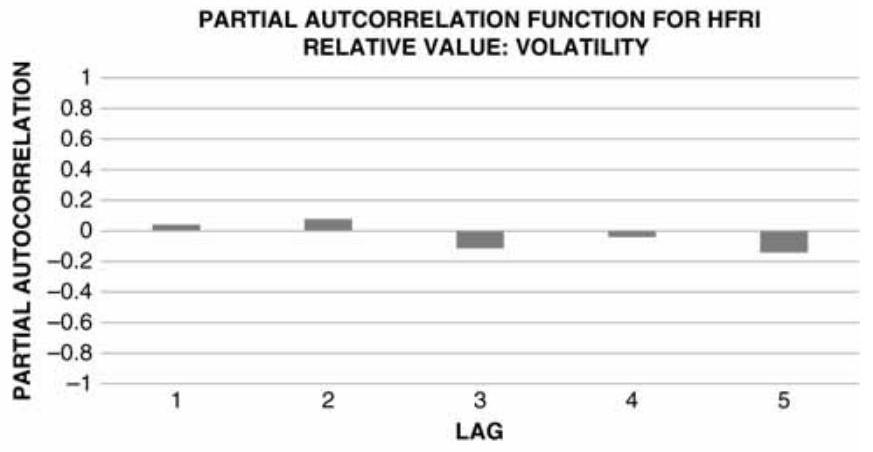
\includegraphics[max width=\textwidth]{2024_04_09_f30d6bff3ec27dfda1e7g-08}
\end{center}

Histogram of HFRX Relative Value: Volatility (Monthly) Jan. 2009-Dec. 2021

Bucket 1: -Infinity $\%<x<-4.4 \%$

Bucket 2: $-4.3 \%<x<-3.7 \%$

Bucket 3: $-3.6 \%<x<-2.9 \%$

Bucket 4: $-2.8 \%<x<-2.1 \%$

Bucket 5: $-2.0 \%<x<-1.4 \%$

Bucket 6: $-1.3 \%<x<-0.6 \%$

Bucket 7: $-0.5 \%<x<0.9 \%$

Bucket $8: 1.0 \%<x<1.7 \%$

Bucket 9: $1.8 \%<x<2.5 \%$

Bucket 10: $2.6 \%<x<3.3 \%$

Bucket 11: $3.9 \%<x<4.0 \%$

Bucket 12: $4.1 \%<x<4.9 \%$

Bucket 13: $5.0 \%<x<$ Infinity \%

\section*{Statistical Summary of Returns}
Key observations on relative value volatility returns that are consistent with economic reasoning are an essential component of knowledge and include the following.

\begin{enumerate}
  \item The historical return distribution of HFRI Relative Value: Volatility exhibited modestly greater left skew and quite high excess kurtosis relative to global equities.

  \item Volatility of returns was very substantially lower than that of world equities.

  \item Returns exhibited modest positive first-order autocorrelation.

  \item Maximum drawdown was very much better than that observed for global equities.

\end{enumerate}

\end{document}